\documentclass[a4paper, 12pt, twoside]{article}
\usepackage[hungarian]{babel}
\usepackage{ae,aecompl}
\usepackage[T1]{fontenc}
\usepackage[utf8]{inputenc}
\usepackage{textcomp}
\usepackage{pgfplots}
\usepackage{anysize}
% left right up down
\marginsize{3.2cm}{2.8cm}{2cm}{2cm}
\usepackage{setspace}
\setstretch{1.2}
\frenchspacing
\pgfplotsset{compat=newest}
%\pagestyle{empty}
\usepgfplotslibrary{ternary}
\usepackage{chemfig}
\usepackage{gensymb}
\usepackage{fancyhdr}
\usepackage{enumerate}
\usepackage{amsmath}
\usepackage{upgreek}
\numberwithin{equation}{section}
\numberwithin{figure}{section}
\numberwithin{table}{section}
\hyphenation{hő-mér-sék-let-füg-gé-sét}

\renewcommand\footrule{\begin{minipage}{1\textwidth}
%\hrule width \hsize height 2pt \kern 1mm \hrule width \hsize   
\hrule width \hsize height 1pt   
\end{minipage}\par}%

\renewcommand\headrule{
\begin{minipage}{1\textwidth}
%\hrule width \hsize \kern 1mm \hrule width \hsize height 2pt 
\hrule width \hsize height 1pt 
\end{minipage}}%

\pagestyle{fancy}
\fancyhf{}
%\fancyhead[LE,RO]{\leftmark}

%\setlength{\footskip}{40pt}

%\pagestyle{fancy}
%\fancyhf{}
%\usepackage{lastpage}
%\rfoot{Page \thepage \hspace{1pt} of \pageref{LastPage}}
%\lhead{\thesection}
%\cfoot{\itshape\textcolor{gray}{Fizikai Kémia gyakorlatok gyógyszerészeknek}}

\setcounter{tocdepth}{1}
%\thispagestyle{empty}
\title{Physical chemistry laboratory practice for pharmacy students}
\author{\emph{written by:} \\ Barna Kovács \\ Sándor Kunsági-Máté \\ Géza Nagy \\ \\ \emph{translated by:} \\ András Kiss}
\date{}
 
\begin{document}
%\clearpage\maketitle
%\thispagestyle{empty}
%\newpage 
%\tableofcontents
%\newpage

%\fancyhead[LE,RO]{Drug decomposition -- ,,GYB''}
\fancyhead[LO,RE]{\thesection}
\fancyfoot[LE,RO]{\thepage}
\fancyfoot[RE,LO]{\emph{Physical chemistry lab. practice for pharmacy students}}

%\setcounter{section}{7}
\section{Investigating the temperature dependence of drug decomposition}
\subsection{Introduction}

During this practice we study the pseudo first-order hydrolysis reaction of acetilsalicilic acid.
The rate constant of a first-order reaction can be written as:

\begin{equation}
\label{eq:divider}
        k
        =
        \frac
                {1}
                {t}
	\ln
	\frac{z}{z-x}
\end{equation}

where $t$ is time, $z$ is the initial concentration of the reagent, $x$ is the concentration of the product at time $t$.

The reaction rate depends on temperature, which is stated in the \emph{Arrhenius law}:

\begin{equation}
\label{eq:divider}
        \frac
                {d\ln k}
                {dT}
	=
	\frac
		{E}
		{\mathrm{R}T^2}
\end{equation}

after integration:

\begin{equation}
\label{eq:divider}
        k
        =
	A
	e^{-E/( \mathrm{R} T)}
\end{equation}

and

\begin{equation}
\label{eq:divider}
        \lg k
        =
        \lg A
	-\frac{E}{2.303 \mathrm{R}T}
\end{equation}

$A$ is the preexponential factor, $E$ is the activation energy, and R is the universal gas constant (R$ = 8.314$ J/Kmol). The factor 2.303 is the conversion form ln to lg.
Activation energy can be obtained graphically if we take the slope of the function $\lg k - 1/T$ and multiply it by 2.303 $\times$ 8.314. The dimension in this case for $E$ is J/mol.
If we measure $k$ on two different temperatures ($k_1$ and $k_2$ on $T_1$ and $T_2$ temperature), activation energy can be calculated as follows:

\begin{equation}
	E
	=
	2.303
	\times
	8.314
	\lg
	\frac{k_1}{k_2}
	\frac{T_1 T_2}{T_1-T_2}
\end{equation}

\subsection{Practice procedures}

Alkaline hydrolysis of acetylsalicylic acid (Fig. \ref{fig:salicilsav}) is a pseudo first-order reaction. 
\begin{figure}
\centering
\schemedebug{false}
\schemestart
	\footnotesize \chemname{\chemfig{*6(-=-(-O-[::-60]([::-60]=O)-)=(-(-[::-60]OH)=[::60]O)-=)}}{acetylsalicylic acid}
	\footnotesize \+
	\footnotesize \chemfig{OH^{-}}\arrow(.mid east--.mid west){->[k][]}
	\footnotesize \chemname{\chemfig{*6(-=-(-OH)=(-([::-60]-OH)=[::60]O)-=)}}{salicylic acid} + CH$_3$COO$^-$
\schemestop
\caption{Alkaline hydrolysis of acetylsalicylic acid.}
\label{fig:salicilsav}
\end{figure}
The reaction is quite slow on room temperature, therefore we conduct our measurements at a higher temperature.
To determine the rate constant $k$, we need to know the change in concentration of the reactants or the products as a function of time.
In this practice, we will use spectrophotometry after forming an Fe$^{3+}$ salicilate complex by adding FeCl$_3$ to the samples. The complex has a deep violet color, and its absorbance is directly proportional to the concentration of the complex, therefore to the concentration of the product salicilate as stated by \emph{Lambert-Beer's law}:

\begin{equation}
\label{eq:beer}
        A
        =
	\epsilon
	l
	c
\end{equation}

where A is absorbance, $\epsilon$ is the molar decadic absorption coefficient, $l$ is the length of the solution block the light is passing through, and $c$ is the concentration.
We take known volumes of samples from the alkaline reaction vessel, and suddenly decrease [OH$^-$] and temperature by adding NaOH and putting the samples on ice.
If the measured absorbance is above 2 A.U., dilution is necessary, since over this value the relationship between $c$ and $A$ is not linear anymore. To determine the product concentration at $t = \infty$ (which equals to the reactant concentration at $t = 0$), we take samples at the and of the practice. We carry out the measurements at two different temperatures, determined by the instructor (usually 313 and 353 K).

Pulverize an \emph{Aspirin} tablet in a mortar with the help of a pestle, dissolve it a small amount of deionized water, then filter it into a 100 cm$^3$ measuring flask, and fill it up to 100 cm$^3$. This will be the stock solution. The stock solution obtained in this way will be most likely saturated\footnote{An \emph{Aspirin} tablet has 500 mg acetylsalicylic acid in it, and its solubility in water is 2 - 4 g / L, depending on temperature.}

\textbf{Starting and following the reaction:}

\begin{enumerate}[(a)]
\item Determining the initial concentration $z$ of acetylsalicylic acid. Pipette 2-2 cm$^3$ sample from the stock solution into two Erlenmeyer flasks with bottlecaps (low and high temp.), and add 3-3 cm$^3$ 0.25 M NaOH solution to them. Put them into the two thermostats after labeling them. At the end of the practice we stop the reaction. It should be complete, but we should treat these solutions as the others to rule out any artifacts. ,,Stop the reactions'' by adding 2-2 cm$^3$ 0.25 M HCl solution and 3-3 cm$^3$ FeCl$_3$, then fill the flasks up to 100 cm$^3$ with deionized water.

\item Determining concentration $x$ at time $t$. Put one half of the remaining stock solution into an Erlenmeyer and the other half into another Erlenmeyer flask. Close the flasks, label them, and put them into their respective thermostats. Add 5 cm$^3$ buffer solution (ask the technician), and start a stopwatch. By adding the buffer solution the reaction starts ($t$ = 0). Without taking out the flask, take 2 cm$^3$ samples from them at 15, 20, 25, 30 and 35 minutes after the reaction has started, and put them into separate, labeled 25 cm$^3$ measuring flasks you prepared beforehand. Prepare them by adding 0.5 cm$^3$ 0.25 M HCl solution (this will stop the \emph{alkaline hdydrolysis}), and 0.5 cm$^3$ 0.1 M FeCl$_3$ solution (to form the complex and make the product visible for spectrophotometry). Fill the remaining volume in the 25 cm$^3$ flasks with deionized water. Start the two reactions by shifting one by $1 - 2$ minutes, so you don't have to take samples at the same time from the two reactions.
\end{enumerate}

\textbf{Measuring absorbance and calculating concentration}. Both the initial and the instantaneous concentration at time $t$ will be measured spectrophotomertically. Find the users manual next to the instrument, or ask the instructor to help. To calculate the concentration from absorbance use the factor $b = 8.3~(mol/dm^3) / AU$. This is the concentration of the theoretical solution, whose absorbance is 1 AU, if $d = 1~cm$, where $d$ is the length of solution block in the path from source to detector.

\subsection{Results to submit}

\begin{enumerate}
\item Measured and calculated data in table (use table \ref{table:tablazatos} as reference).
\item Calculate the rate constants (table \ref{table:seb}.) for both temperatures, and calculate standard deviation\footnote{Standard deviáció, $s=\sqrt{\frac{\Sigma(x_i-\overline{x})^2}{n-1}}$}.
\item From the temperature dependence of the rate constant, calculate the rate constant for 20 $\celsius$-on (293 K) graphically by plotting $\lg k$ as a function of $1/T$.
\item Calculate $E$ and $A$ by substituting into the integrated form of the Arrhenius equation:
	\begin{enumerate}
		\item E [kJ mol$^{-1}$]
		\item $\lg$ A [$s^{-1}$]
		\item A [s$^{-1}$]
	\end{enumerate}
\end{enumerate}

\begin{table}[h!]
\caption{Measured and calculated data.}
\centering
T = ... K, $z$ = ... mg/100 cm$^3$
\begin{tabular}{|c|c|c|c|c|c|}
\hline
reaction time, s&dilution&A&x, mg / 100 cm$^3$ &(z-x), mg / 100 cm$^3$ & $k$, s$^{-1}$ \\
\hline
... & ... & ... & ... & ... & ... \\
\end{tabular}
\label{table:tablazatos}
\end{table}

\begin{table}[h!]
\caption{Temperature dependence of the rate constant.}
\centering
\begin{tabular}{|c|c|c|c|c|}
\hline
T, K& 1/T & $\overline{k}$ (average), s$^{-1}$ & $\lg k$ & standard deviation \\
\hline
... & ... & ... & ... & ... \\
\end{tabular}
\label{table:seb}
\end{table}

\vfill

%Updated and translated by András Kiss in 2016.

%\newpage
%\clearpage
%\fancyhead[LE,RO]{Ionselective electrodes -- ,,SZEL''}
\fancyhead[LO,RE]{\thesection}
\fancyfoot[LE,RO]{\thepage}
\fancyfoot[RE,LO]{\emph{Physical chemistry lab. practice for pharmacy students}}

%\setcounter{section}{7}
\section{Determination of selectivity coefficient of ion-selective electrode}
\subsection{Introduction}

Ion-selective electrodes are potentiometric sensors, that allow the selective determination of the activity of certain ions.
They are widely used in the clinical diagnostics for routine measurements: automatic blood analisators measure the Na$^+$ and K$^+$-ion activity in blood samples. One more example is the determination of F$^-$-ion in tap water, even if there are interfering ions such as Cl$^-$ or OH$^-$. Their function is based on a selective membrane, which can be ionophore based (Na$^+$ and K$^+$), or lattice vacancy based (F$^-$). An example for the latter is the F$^-$ ion-selective electrode, which is based on a europium doped lanthanum fluoride crystal.

The equation that describes the behaviour of these electrodes is the Nernst-equation:

\begin{equation}
\label{eq:nernst}
	E
	=
	E^0
	+\frac{RT}{z_i F}
	ln(a_i)
\end{equation}

where $z_i$ is the signed valence of the primary ion (the ion that the electrode is selective to), $a_i$ is its activity.
According to the equation, for cation elective electrodes the electrode potential ($E$) is increasing with increasing actvity, and for anion selective ones, it decreases.
Because of deviations from the theoretical behaviour, in practice, we use the following, experimental equation:

\begin{equation}
\label{eq:exp}
	E
	=
	E^0
	\pm S ln(a_i)
\end{equation}

where $S$ is the slope of the linear part of the electrode calibration curve, which can be measured.
In real, multi-component samples, the potential of the ion-selective electrodes is influenced by the so-called \emph{interfering ions}, but in fact, more or less by every ion in the sample to some (small) extent.
For this reason, using eqs. \ref{eq:nernst} and \ref{eq:exp} will introduce error during evaluation.
To take into account these deviations we use the concept of \emph{selectivity coefficient} ($k_{pot}$). With this we can rewrite the equations as such: 

\begin{equation}
\label{eq:nikolsky}
E=E^0 + \frac{RT}{z_iF} \ln \left [ a_i + \sum_{j} \left ( k_{ij}a_j^{z_i/z_j} \right ) \right ]
\end{equation}

This is the Nikolsky equation. $a_j$ is the activity of the $j$th interfering ion, $z_j$ is its charge, $k_{pot}$ $i, j$ is the selectivity coefficient of the $j$th ion.
The selectivity coefficient shows how much more sensitive is the electrode towards the primary ion, then towards to the interfering ion.
For instance, if $k = 10^{-2}$, the activity of the $j$ ion must be hundredfold of the $i$ primary ion to have the same effect on the electrode potential (increase or decrease it to the same extent).
There are two main methods for determining the selectivity coefficient: the mixed and the separate solution methods.

In the mixed solution method, ion activity of the $j$ interfering ion is constant, and we increase the activity $i$ primary ion, and measure the potential response.
After plotting the data fig. \ref{fig:Q}, we find $Q$. Then, we calculate the selectivity coefficient as follows:

\begin{equation}
\label{eq:szel1}
	k_{i,j}^{pot}
	=
	\frac{(a_i^{z_j})_Q}{a_j^{z_i}}
\end{equation}


\begin{figure}
\centering
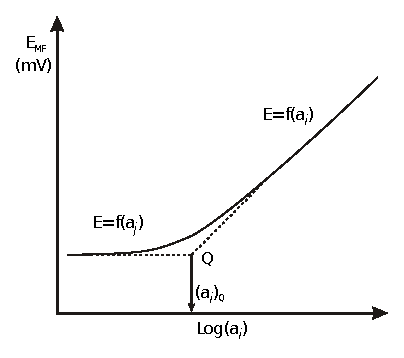
\includegraphics{ion1.eps}
\caption{Using the mixed solution method to determine the selectivity coefficient.}
\label{fig:Q}
\end{figure}

When using the separate solution method, we need to record two calibration curves.
First, at zero interfering ion activity, we make a calibration of primary ion $i$, then at zero primary ion $i$ activity, we make a calibration plot of interfering ion $j$.
After obtaining these two curves, the selectivity coefficient can be obtained as seen in fig. \ref{fig:ion2}, taking either

\begin{enumerate}[(a)]
\item activities corresponding to the same potentials:

\begin{equation}
\label{eq:azonospot}
        k_{i,j}^{pot}
        =
        \frac{a_i}{a_j^{z_i/z_j}}
\end{equation}

\item or potentials corresponding to the same activities:

\begin{equation}
\label{eq:azonosakt}
        \lg k_{i,j}^{pot}
        =
        \frac{(E_2-E_1)zF}{2.303RT}
	=
	\frac{\Delta E}{S}
\end{equation}

\end{enumerate}

There are a number of factors that influence the selectivity coefficient: ionic strength, method, etc...
As it can be seen, from relationships \ref{eq:azonospot} and \ref{eq:azonosakt}, the drawback of the separate solution method is that it assumes, that the valence of the primary and interfering ion is equal, and that the sensitivity towards them is the same.
For this reason, selectivity coefficients obtained with this method are regarded as approximations, and the much better mixed solution method is preferred.

\begin{figure}
\centering
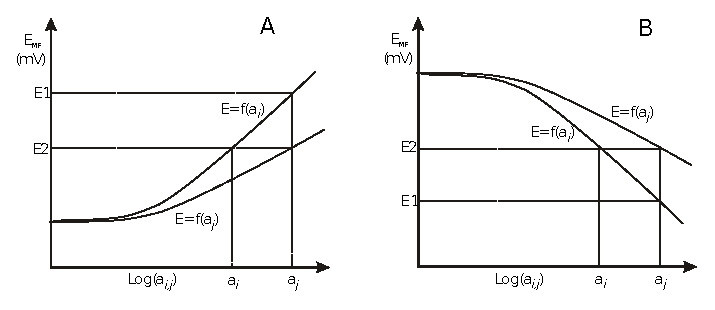
\includegraphics{ion2.eps}
\caption{Determining the selectivity coefficient with the separate solution method for positive (A) and negative (B) ions.}
\label{fig:ion2}
\end{figure}

\subsection{Practice procedures}
The purpose of this practice is to study the function of potassium or fluoride ion-selective electrodes (ask the instructor which one).
Your first task is to prepare a dilution series of soluions of the primary ion. Use salts KCl or NaF.
Prepare 100 ml 10$^{-2}$ mol$\cdot$dm$^{-3}$ solution using a salt of the primary ion. 
Then make a tenfold dilution by taking out 10 ml from this solution, and putting it in another, clean 100 ml measuring flask. Fill it up to 100 ml with deionized water. Continue making dilution by always using the previous solutions, until you reach a concentration of 10$^{-6}$ mol$\cdot$dm$^{-3}$. 
Pour a small amount of each into separate, labeled beakers, so that the electrodes can submerse into them with their active area.
Then start with the most dilute solution by putting the measuring and the reference electrodes into it. Wait 1 minute, and write down the potential.
Move on to the next solution (10$\times$ more conc.), wait another 1 minute, and record the data.
Carry out measurements in all five solutions advancing from dilute to concentrated, repeat it altogether 3 times. Carefully rinse the electrodes between series.

\subsubsection{Determining the selectivity coefficient using the separate solution method}
Repeat the previous procedure, but use a salt of the interfering ion to prepare the first solution, the do the dilutions. It's important to use deionized water free of potassium, sodium, chloride and fluoride ions as much as possible. Ask the technician for ultrapure water. 

\subsubsection{Determining the selectivity coefficient using the mixed solution method}
For this method prepare another dilution series by using a salt of the primary ion, but instead of deionized water, use a 10$^{-2}$ M solution of the interfering ion as solvent. In this way, the interfering ion concentration will be constant in all of the solutions, but the primary ion concentration will vary just like in the first experiment.

\subsection{Evaluation}
\begin{enumerate}
\item Find the activity coefficients for the primary and interfering ions online, and calculate the activities from the concentrations.

\item Plot the $\lg a_i$ -- $E$ functions as seen in the diagrams above. 

\item Determine the slope of the linear part by linear fitting for each graph.

\item Determine the lower limit of detection of the electrode towards the primary ion ($Q$ when there is no interfering ion).

\item Calculate the selectivity coefficients using all 3 methods (1 mixed solution method and 2 separate solution methods).

\item For the separate solution method, plot the two curves in the same diagram.
\end{enumerate}

\subsection{Results to submit}
Lower limit of detecction towards the primary ion, 2 selectivity coefficients from the separate solution method, and 1 from the mixed solution method.
Five calibration diagrams, each with linear fits on the linear section.

\vfill
%\center
%Updated and translated by András Kiss assistant lecturer 2016.

%\newpage
%\fancyhead[LE,RO]{Determination of pK with conductometry -- ,,PKVEZ''}
\fancyhead[LO,RE]{\thesection}
\fancyfoot[LE,RO]{\thepage}
\fancyfoot[RE,LO]{\emph{Physical chemistry laboratory practice}}

%\setcounter{section}{1}
\section{Determination of dissociation constants of weak acids with conductometry}
\subsection{Introduction}
According to Ohm's law, the current passing through between two points and the potential difference between those two points are in linear relationship:

\begin{equation}
\label{eq:ohm}
	U
	=
	I
	\cdot
	R
\end{equation}

where $R$ is the factor of proportionality, called \textbf{electrical resistance}. Its dimension is ohm ($\ohm$).

Specific resistance is the longitudinal resistance of a conductor which is 1 m long and has a cross section of 1 m$^2$ (1 mm$^2$ in practice). 

In electrochemistry it is often more simple to use the reciprocal of these quantities. The reciprocal of resistance is conductivity, its dimension is Siemens, S = 1/$\ohm$. The reciprocal of specific resistance is specific conductivity. The specific conductivity of an electrolyte is the conductivity we measure if the two electrodes have a surface area of 1 cm$^2$, they are 1 cm apart, they are made of an inert metal (gold, platinum), and they are submersed in the electrolyte. Its dimension is S $\cdot$ cm$^{-1}$. It depends on concentration, temperature, and it's a unique property of every material.

Molar specific conductivity ($\Lambda _m$) is the ratio of the specific conductivity and the concentration:

\begin{equation}
\label{eq:lambdam}
        \Lambda_m
        =
        \frac
		{\kappa 1000 }
		{c}
	=
	\kappa V
\end{equation}

where $c$ is concentration (mol$\cdot$dm$^{-3}$), and $V$ is dilution.

Kohlrausch found that the limiting molar conductivity (molar conductivity of an infinitely dilute solution) of anions and cations are additive: the conductivity of a solution of a strong electrolyte is equal to the sum of conductivity contributions from the cation and anion:

\begin{equation}
\label{eq:kohlrausch2}
	\Lambda _m^0
	=
	\lambda _a^0 \nu _a z_a + \lambda _k^0 \nu _k z_k
%	/1000
\end{equation}

where $z_a, z_k$ are the valence of the ions, $\nu _a, \nu _k$ are stochiometric factors, $\lambda _a^0$ and $\lambda _k^0$ are the limiting molar conductivities for the anions and the cations.

The conductivity of weak electrolytes can be described as follows:

\begin{equation}
\label{eq:lambdam}
        \lambda_c
        =
        \alpha
	\lambda_0
\end{equation}

where $\alpha$ is the degree of dissociation, $\lambda _0$ is the limiting molar conductivity.
The dissociation constant $K_d$ of a weak acid can be calculated from its concentration and its degree of dissociation:

\begin{equation}
\label{eq:kd}
        K_d
        =
        \frac{\alpha^2 c}{1-\alpha}
\end{equation}

It is worth noting however, that $K_d$ -- based on the Debye-Hückel theory -- depends on the permittivity of the media and temperature.

If we express $\alpha$ from \ref{eq:lambdam}, we get \emph{Ostwald's law of dilution}:

\begin{equation}
\label{eq:ostwald}
        K_d
        =
        \frac{\lambda_c^2 c}{\lambda_0^2 - \lambda_0\lambda_c}
\end{equation}

That means we can determine $K_d$ from conductometric measurements. $\lambda_c$ can be measured directly, while $\lambda_0$ can be obtained with the following method. By rearranging eq. \ref{eq:ostwald} we get

\begin{equation}
\label{eq:ostwald2}
        \frac{1}{\lambda_c}
        =
	\lambda_c
	c
	\frac{1}{K_d \lambda_0^2}
	+\frac{1}{\lambda_0}
\end{equation}

If we plot $1/\lambda_c$ as a function of $\lambda_c c$ (which is nothing but $\kappa$), we get a straight line whose y interception is $1/\lambda_0$. And knowing $\lambda_c$ and $\lambda_0$ we can calculate $K_d$.

Additionally, we have to consider these:

\begin{enumerate}[(a)]
\item The solvent also contributes to the conductivity of the solution. Therefore we substract the conductivity of the pure solvent ($G_{\text{solvent}}$) from each measurement carried out in the solutions of that solvent.

\item In practice, we don't use the conductivity cell from the definition of specific conductivity. Instead, the more practical ,,bell electrodes'' are used. To obtain specific conductivity from the conductivity values measured with these cells, we multiply every value with the cell constant $C$ (dimension:  m$^{-1}$ or cm$^{-1}$).

The cell constant shows the relationship between solution with a known specific conductivity ($\kappa_{ref}$) and the conductivity measured with cell used in practice ($G_{\text{measured}}$):

\begin{equation}
\label{eq:c}
	C
	=
	\kappa_{\text{ref}}/G_{\text{measured}}
\end{equation}

\end{enumerate}

Based on this, we can calculate the contribution of solute to the conductivity of the solution: $\kappa_{\text{korr}} = (G_{\text{solution}} - G_{\text{solvent}})C$, where $\kappa_{\text{korr}}$ is the specific conductivity of the solution taking into account that of the solvent and the cell constant.

Therefore, specific molar conductivity of a weak acid is:

\begin{equation}
\label{eq:c}
        \lambda
        =
        \kappa_{korr}
	V
\end{equation}


\begin{figure}[h!]
\centering
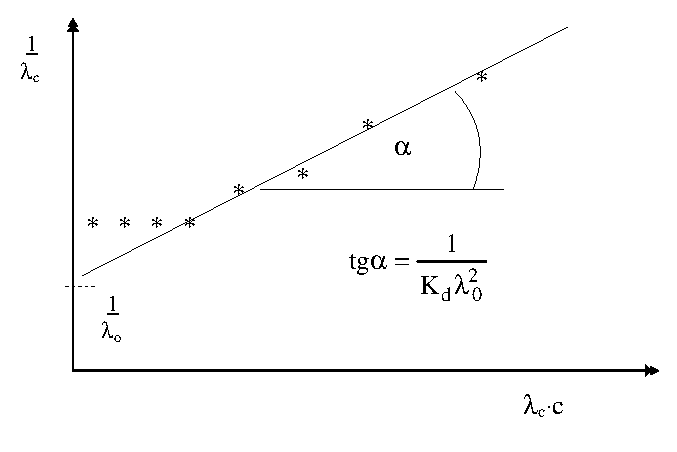
\includegraphics{fig/lambda0.eps}
\caption{Obtaining the limiting molar conductivity ($\lambda_0$).}
\label{fig:}
\end{figure}

\subsection{Practice procedures}

Rinse the electrode of the conductometer several times (4 - 5) with deionized water, the with ultrapure water ($\kappa$ < 1 $\upmu$S/cm). Ask the technician for ultrapure deionized water.

Prepare 20 v/v\% solution from an alcohol selected by the instructor. Then prepare two weak acid solutions (the weak acid is also selected by the instructor), from the stock solution (1 mol$\cdot$dm$^{-3}$) by pipetting 2.00 cm$^3$ into two 100 cm$^3$ measuring flasks, and then filling one with the 20 v/v\% alcohol solution, the other with ultrapure deionized water up to 100 cm$^3$.

Carry out the conductivity measurements in a measuring cilinder. Pour the water based solution into the cilinder and measure its conductivity. Then, pipette 25 cm$^3$ from the cilinder into a clean 50 cm$^3$ measuring flask, fill it up with ultrapure deionized water (2$\times$ dilution), and measure the conductivity of the new solution after carefully rinsing it with ultrapure deionized water. Repeat the dilution and measurement 3 times. Then do the same with the alcohol based solution, but using the 20 v/v\% alcohol solution for the dilutions and rinsing.

Note and record the temperature measured by the built-in thermometer of the electrode for each measurement.

Finally, measure the conductivity of the solvents as well (for the correction).
Then, to obtain the cell constant, measure the conductivity of 0.01 M KCl solution, and write down the temperature as well. Based on table 

Figure \ref{fig:vez} shows the schematics of a conductometric cell. A well-defined, inert electrode pair is submersed into an electrolyte, and the voltage drop between them is measured. Alternating current is used to avoid polarization and electrolysis.

\begin{figure}
\centering
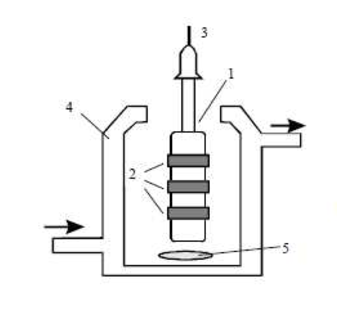
\includegraphics{fig/cond.eps}
\caption{Schematics of a conductometric cell. 1 - ,,bell electrode'', 2 - platinized platinum rings, 3 - electrical connection, 4 - double walled vessel, 5 - magnetic stirrer.}
\label{fig:vez}
\end{figure}

\subsection{Evaluation}

\begin{enumerate}
\item Calculate the cell constant.
Present the recorded data in such a table:

\begin{table}[!h]
\centering
\begin{tabular}{|c|c|c|c|c|c|c|c|}
\hline
c (mol $\cdot$ dm$^{-3}$) & G$_{\text{measured}}$ & $\kappa_{\text{korr}}$ (S $\cdot$ cm$^{-1}$) & $\lambda_c$ & $1/\lambda_c$ & $\lambda_c c$ & $\alpha$ & $K_d$ \\
\hline
... & ... & ... & ... & ... & ... & ... & ... \\
\end{tabular}
\label{table:vez}
\end{table}

\item Determine $\lambda_0$ graphically. Knowing $\lambda_c$ and $\lambda_0$, calculate $\alpha$ and $K_d$ for each concentration.

\end{enumerate}



%\newpage
\section{Gyengesav disszociációs állandójának meghatározása vezetés mérésével}
\subsection{Bevezetés}
Az elektromos ellenállás anyagi tulajdonság.
Ohm törvénye értelmében egy anyagon átfolyó elektromos áram erősége ($I$) és az áramot létrehozó feszültség ($U$) között egyenes arányosság van:

\begin{equation}
\label{eq:ohm}
	U
	=
	I
	\cdot
	R
\end{equation}

ahol az $R$ arányossági tényezőt az illető anyag ellenállásának nevezzük, mértékegysége az ohm ($\ohm$).
Fajlagos ellenálláson az 1 m hosszú, 1 m$^2$ (a gyakorlatban 1 mm$^2$) keresztmetszetű vezetőn az 1 amper intenzitású áram létrehozásához szükséges feszültség és az áram hányadosát értjük.

Az elektrokémiában több szempontból előnyös, ha a fenti mértékegységek reciprokait használjuk: az ellenállás reciprokát vezetésnek (mértékegysége a Siemens, S = 1/$\ohm$), a fajlagos ellenállás reciprokát fajlagos vezetésnek nevezzük.

Elektrolitok oldatainak fajlagos vezetésén ($\kappa$) az 1 cm távolságban, párhuzamos, 1-1 cm$^2$ felületű elsőrendű (inert fém, pl. arany vagy gyakrabban platina) vezetőből készült elektródok között elhelyezkedő folyadékkocka vezetését értjük, mértékegysége S $\cdot$ cm$^{-1}$.
A fajlagos vezetés függ az elektrolit anyagi minőségétől, koncentrációjától, valamint a hőmérséklettől.
Moláris fajlagos vezetésen ($\Lambda _m$) a fajlagos vezetés és a koncentráció hányadosát értjük. Ez alapján

\begin{equation}
\label{eq:lambdam}
        \Lambda_m
        =
        \frac
		{\kappa 1000 }
		{c}
	=
	\kappa V
\end{equation}

ahol $c$ az oldat koncentrációja (mol$\cdot$dm$^{-3}$) és $V$ a hígítás.
%A vezetés szoros kapcsolatban van az ionok mozgékonyságával: ha ugyanis a mérő elektródra feszültséget kapcsolunk, az elektrolitban ionvándorlás indul meg.
%A vándorlás sebessége függ az elektromos térerő nagyságától, ezért a vándorlási sebességet 1 V/cm térerőre vonatkoztatjuk.
%Az 1 V/cm térerő hatására másodpercenként megtett utat az ion relatív mozgékonyságának ($u$) nevezzük.
Mivel egy biner elektrolitban mind az anionok, mind a kationok hozzájárulnak a vezetéshez, erős elektrolitok híg oldatainak fajlagos moláris vezetését az \emph{ionok független vándorlásának törvénye} írja le:

\begin{equation}
\label{eq:kohlrausch2}
	\Lambda _m^0
	=
	\lambda _a^0 \nu _a z_a + \lambda _k^0 \nu _k z_k
%	/1000
\end{equation}

ahol $z_a, z_k$: ionok töltésszáma; $\nu _a, \nu _k$: sztöchiometriai konstansok; $\lambda _a^0$ illetve $\lambda _k^0$ az anionok és a kationok végtelen hígításra vonatkozó moláris fajlagos vezetése.
Gyengeelektrolitok vezetése

\begin{equation}
\label{eq:lambdam}
        \lambda_c
        =
        \alpha
	\lambda_0
\end{equation}

formában adható meg, ahol $\alpha$ a disszociáció foka, $\lambda _0$ a végtelen hígítású oldat moláris fajlagos vezetése.
%Ha a gyengeelektrolit koncentrációja kicsi, az ionmozgékonyságok csak a hőmérséklettől függenek, a koncentrációtól nem.
Egy AH gyengesav disszociációs állandója ($K_d$) kiszámítható a koncentráció és a disszociáció fokának ismeretében

\begin{equation}
\label{eq:kd}
        K_d
        =
        \frac{\alpha^2 c}{1-\alpha}
\end{equation}

Érdemes megjegyezni azonban, hogy a disszociációs állandó adott hőmérsékleten függ - a Debye-Hückel elmélet alapján - a közeg permittivitásától is.
Ha a \ref{eq:lambdam} egyenlet $\alpha$-ra rendezett alakját behelyettesítjük ez utóbbi egyenletbe, a gyengeelektrolitok disszociációjára Ostwald által megállapított összefüggéshez jutunk (\emph{Ostwald féle hígítási törvény}):

\begin{equation}
\label{eq:ostwald}
        K_d
        =
        \frac{\lambda_c^2 c}{\lambda_0^2 - \lambda_0\lambda_c}
\end{equation}

A disszociációs állandó értékét tehát vezetésméréssel meghatározhatjuk. 
$\lambda_c$ közvetlenül mérhető, míg $\lambda_0$ értékét az alábbiak szerint határozhatjuk meg:
A \ref{eq:ostwald} egyenlet átrendezésével

\begin{equation}
\label{eq:ostwald2}
        \frac{1}{\lambda_c}
        =
	\lambda_c
	c
	\frac{1}{K_d \lambda_0^2}
	+\frac{1}{\lambda_0}
\end{equation}

kifejezést kapjuk.
Ha ábrázoljuk $1/\lambda_c$-t $\lambda_c c$, azaz $\kappa$ függvényében, egyenest kapunk, melynek tengelymetszete $1/\lambda_0$. $\lambda_c$ és $\lambda_0$ ismeretében pedig $K_d$ értéke már kiszámítható.
A mérések kivitelezésekor a következőket kell figyelembe vennünk:
\begin{enumerate}[(a)]
\item Az oldat mért vezetéséhez az oldott anyag mellett az oldószer is hozzájárul.
Híg oldatok esetén ezért külön méréssel meghatározzuk az oldószer vezetését ($G_{\text{oldószer}}$) és ezt az értéket levonjuk az oldat esetében mért vezetés értékéből.

\item Az újabban használatos elektródok geometriája és elrendezésük eltérnek a fajlagos vezetés definíció szerinti meghatározásánál leírtaktól, ezért a mérőelektródot kalibrálni kell.
Az eltérés a mérést nem befolyásolja, mivel az eltérés az úgynevezett cellaállandó - mint kalibrációs paraméter - segítségével figyelembe vehető.
A cellaállandó (jele $C$, egysége m$^{-1}$ vagy cm$^{-1}$) megmutatja egy ismert fajlagos vezetésű oldat ($\kappa_{ref}$) és az adott mérőcellával ezen oldaton mért vezetés ($G_{\text{mért}}$) közötti kapcsolatot:

\begin{equation}
\label{eq:c}
	C
	=
	\kappa_{\text{ref}}/G_{\text{mért}}
\end{equation}

\end{enumerate}

Ezek alapján az oldat hozzájárulását a vezetéshez a következőképpen kapjuk meg: $\kappa_{\text{korr}} = (G_{\text{oldat}} - G_{\text{oldószer}})C$,
ahol $\kappa_{\text{korr}}$ az oldatnak a cellaállandóval és az oldószer fajlagos vezetésével korrigált értéke, $C$ a cellaállandó (nem tévesztendő össze a koncentrációval, melyet $c$-vel jelölünk).
Ezek alapján a gyengesav oldat moláris vezetése:

\begin{equation}
\label{eq:c}
        \lambda
        =
        \kappa_{korr}
	V
\end{equation}

ahol V a hígítás.

\begin{figure}
\centering
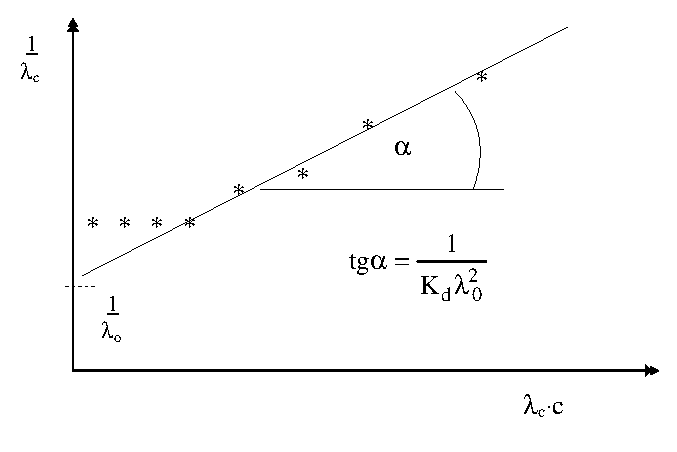
\includegraphics{fig/lambda0.eps}
\caption{Végtelen higítású oldat vezetésének ($\lambda_0$) meghatározása.}
\label{fig:}
\end{figure}

\subsection{A gyakorlat leírása}

A konduktométer harangelektródját többször (4 - 5) öblítsük át desztillált vízzel majd kis részlet 1 $\upmu$S/cm-nél kisebb fajlagos vezetésű vízzel, melyet külön edényben a technikustól kell kérni.
A gyakorlatvezető által kijelölt alkohollal (metanol, etanol vagy propanol) készítsünk 20 v/v\%-os oldatot.
A kijelölt 1 mol$\cdot$dm$^{-3}$ koncentrációjú gyengesav törzsoldatából pipettázzunk két száraz 100 cm$^3$-es mérőlombikba 2.00 cm$^3$-t, majd töltsük jelre az első lombikot vezetőképességi vízzel, a másikat a 20\%-os alkohol oldattal.
A mérést mérőhengerben végezzük.

Töltsük először a vizes hígítású oldatot a mérőedénybe, és mérjük meg a vezetését.
Ezután 25 cm$^3$-t pipettázzunk ki az oldatból és 50 cm$^3$-es mérőlombikban hígítsuk kétszeresére.
Az elektród gondos leöblítése után mérjük ezen oldat vezetését is.
%Az oldat vezetését leghelyesebb úgy meghatározni, hogy az elektród bemerítésétől 5 percen át 30-60 másodpercenként észleljük és feljegyezzük a cellában jelentkező vezetés értékeket.
A kétszeres hígítást még 3-4-szer megismételjük, minden alkalommal mérve a vezetést.

Ismételjük meg a méréseket az alkoholt tartalmazó oldatokkal is úgy, hogy a hígítások során bidesztillált víz helyett a mérőlombikot az alkoholos oldattal töltjük mindig jelre.

Minden esetben jegyezzük fel a mért oldat hőmérsékletét is (a vezetőképességmérő írja az elektródba épített hőmérő által mért hőmérsékletet).
%A mérőcellában egy-egy oldatot legalább 25 percig kell termosztálni.
%A rendelkezésre álló idő rövidsége miatt a legcélszerűbb, ha a sorozat következő, már meghígított tagját főzőpohárban előre a termosztátba helyezzük, így csökkentve a két mérés közti várakozási időt.

Végül mérjük meg mind a hígításokhoz használt vezetőképességi víz, mind az alkohol oldat vezetését, melyekkel mérési eredményeinket korrigálnunk kell.
Ezután határozzuk meg 0.1 és 0.01 M KCl oldatok felhasználásával a cellaállandó értékét úgy, hogy cellakonstansként a két mérésből számolt értékek átlagát fogadjuk el.

A \ref{fig:vez}. ábra egy vezetőképesség mérésére szolgáló cella felépítését mutatja.
A mérendő oldatba egy geometriailag jól definiált, indifferens elektródpárt merítünk és az ezen létrejövő feszültségesést mérjük.
A konduktometria gyakorlatban az elektrolízis, ill. az elektromos polarizáció csökkentése, ill. kiküszöbölése érdekében váltóárammal végezzük a mérést.

\begin{figure}
\centering
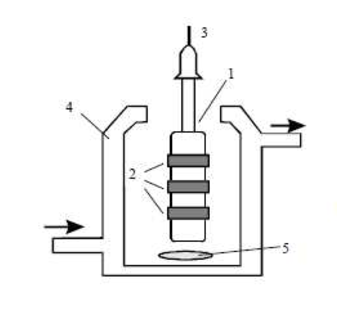
\includegraphics{fig/cond.eps}
\caption{Vezetőképesség mérésére szolgáló cella felépítése. 1 - harangelektród, 2 - Pt korommal bevont gyűrűk, 3 - elektromos elvezetés, 4 - kettős falú temperálható edény, 5 - mágneses keverő.}
\label{fig:vez}
\end{figure}



\subsection{A mérési eredmények kiértékelése}

\begin{enumerate}
\item Számítsuk ki a cellaállandó értékét.
A mérési eredményeket a vizes és az alkoholos sorozatnál is foglaljuk táblázatba:

\begin{table}[!h]
\centering
\begin{tabular}{|c|c|c|c|c|c|c|c|}
\hline
c (mol $\cdot$ dm$^{-3}$) & G$_{\text{mért}}$ & $\kappa_{\text{korr}}$ (S $\cdot$ cm$^{-1}$) & $\lambda_c$ & $1/\lambda_c$ & $\lambda_c c$ & $\alpha$ & $K_d$ \\
\hline
... & ... & ... & ... & ... & ... & ... & ... \\
\end{tabular}
\label{table:vez}
\end{table}

\item Határozzuk meg grafikusan $\lambda_0$ értékét, $\lambda_c$ és $\lambda_0$ ismeretében pedig minden koncentrációra számítsuk ki $\alpha$ és $K_d$ értékeit.

\end{enumerate}






\end{document}
